\documentclass[border=3mm,tikz,preview]{standalone}
\usepackage[utf8]{inputenc}
\usepackage{amsmath,amssymb,amsfonts}
\usepackage{graphicx}
\usepackage{tikz}
\usetikzlibrary{shapes.geometric, arrows.meta, positioning, shadows, calc, fit, backgrounds}
\usepackage{xcolor}
\begin{document}

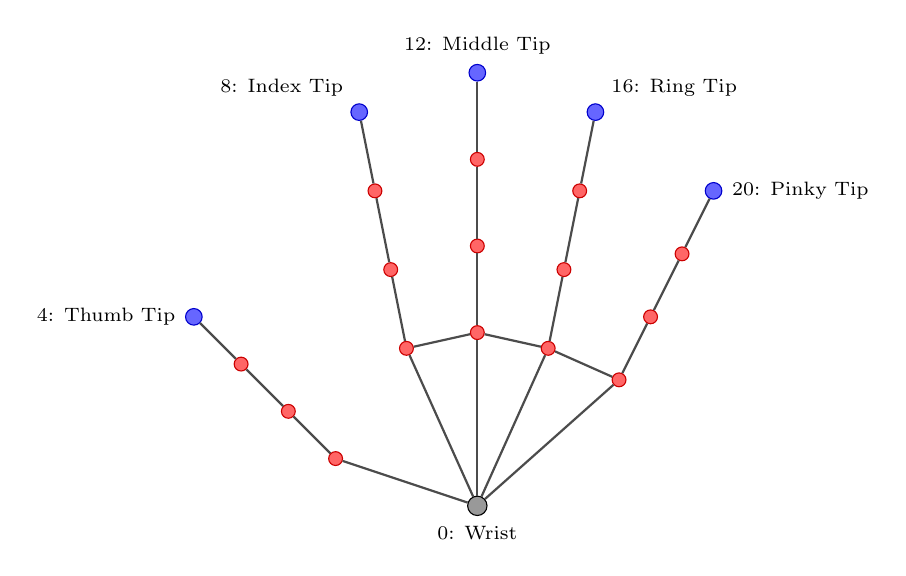
\begin{tikzpicture}[
    joint/.style = {circle, draw=red!80!black, fill=red!60!white, inner sep=0pt, minimum size=5pt},
    tip/.style = {circle, draw=blue!80!black, fill=blue!60!white, inner sep=0pt, minimum size=6pt},
    wrist/.style = {circle, draw=black, fill=gray!80, inner sep=0pt, minimum size=7pt},
    bone/.style = {draw=black!70, thick}
]

% Wrist
\node (J0) [wrist, label=below:{\scriptsize 0: Wrist}] at (0, 0) {};

% Thumb
\node (J1) [joint] at (-1.8, 0.6) {};
\node (J2) [joint] at (-2.4, 1.2) {};
\node (J3) [joint] at (-3.0, 1.8) {};
\node (J4) [tip, label=left:{\scriptsize 4: Thumb Tip}] at (-3.6, 2.4) {};

% Index Finger
\node (J5) [joint] at (-0.9, 2.0) {};
\node (J6) [joint] at (-1.1, 3.0) {};
\node (J7) [joint] at (-1.3, 4.0) {};
\node (J8) [tip, label=above left:{\scriptsize 8: Index Tip}] at (-1.5, 5.0) {};

% Middle Finger
\node (J9) [joint] at (0.0, 2.2) {};
\node (J10) [joint] at (0.0, 3.3) {};
\node (J11) [joint] at (0.0, 4.4) {};
\node (J12) [tip, label=above:{\scriptsize 12: Middle Tip}] at (0.0, 5.5) {};

% Ring Finger
\node (J13) [joint] at (0.9, 2.0) {};
\node (J14) [joint] at (1.1, 3.0) {};
\node (J15) [joint] at (1.3, 4.0) {};
\node (J16) [tip, label=above right:{\scriptsize 16: Ring Tip}] at (1.5, 5.0) {};

% Pinky Finger
\node (J17) [joint] at (1.8, 1.6) {};
\node (J18) [joint] at (2.2, 2.4) {};
\node (J19) [joint] at (2.6, 3.2) {};
\node (J20) [tip, label=right:{\scriptsize 20: Pinky Tip}] at (3.0, 4.0) {};

% Bones Connections
\draw [bone] (J0) -- (J1) -- (J2) -- (J3) -- (J4);
\draw [bone] (J0) -- (J5) -- (J6) -- (J7) -- (J8);
\draw [bone] (J0) -- (J9) -- (J10) -- (J11) -- (J12);
\draw [bone] (J0) -- (J13) -- (J14) -- (J15) -- (J16);
\draw [bone] (J0) -- (J17) -- (J18) -- (J19) -- (J20);
\draw [bone] (J5) -- (J9) -- (J13) -- (J17);

\end{tikzpicture}

\end{document}
